\documentclass[12pt]{exam}

\usepackage[utf8]{inputenc}  % For UTF8 source encoding.
\usepackage{amsmath}  % For displaying math equations.
\usepackage{amsfonts} % For mathematical fonts (like \mathbb{E}!).
\usepackage{upgreek}  % For upright Greek letters, such as \upvarphi.
\usepackage{wasysym}  % For additional glyphs (like \smiley!).
\usepackage{mathrsfs} % For script text (hash families and universes).
\usepackage{enumitem}
\usepackage{graphicx}
% For document margins.
\usepackage[left=.8in, right=.8in, top=1in, bottom=1in]{geometry}
\usepackage{lastpage} % For a reference to the number of pages.
\usepackage[table,xcdraw]{xcolor}
\usepackage{pdfpages}
\usepackage{verbatim}
\usepackage{afterpage}
\usepackage{listings}
\usepackage{color} %red, green, blue, yellow, cyan, magenta, black, white
\definecolor{mygreen}{RGB}{28,172,0} % color values Red, Green, Blue
\definecolor{mylilas}{RGB}{170,55,241}

\newcommand*{\authorname}{Luis A. Perez}

\newcommand*{\duedate}{Wednesday, August 14th}
\newcommand*{\duetime}{11:59 pm}

% Fancy headers and footers
\headrule
\firstpageheader{EE 263\\Summer 2019}{Homework 7 \\ }{Due: \duedate\\at \duetime}
\runningheader{EE 263}{Homework 7}{\authorname}
\footer{}{\footnotesize{Page \thepage\ of \pageref{LastPage}}}{}

% Exam questions.
\newcommand{\Q}[1]{\question{\large{\textbf{#1}}}}
\qformat{}  % Remove formatting from exam questions.

% Useful macro commands.
\newcommand*{\bigtheta}[1]{\Theta\left( #1 \right)}
\newcommand*{\bigo}[1]{O \left( #1 \right)}
\newcommand*{\bigomega}[1]{\Omega \left( #1 \right)}
\newcommand*{\prob}[1]{\text{Pr} \left[ #1 \right]}
\newcommand*{\ex}[1]{\text{E} \left[ #1 \right]}
\newcommand*{\var}[1]{\text{Var} \left[ #1 \right]}

\newcommand*{\norm}[1]{\left\lVert #1 \right\rVert}
\newcommand*{\HH}{\mathscr{H}}   % Family of hash functions.
\newcommand*{\UU}{\mathscr{U}}   % Universe.
\newcommand*{\eps}{\varepsilon}  % Epsilon.


% Custom formatting for problem parts.
\renewcommand{\thepartno}{\roman{partno}}
\renewcommand{\partlabel}{\thepartno.}

% Framed answers.
\newcommand{\answerbox}[1]{
\begin{framed}
\hspace{\fill}
\vspace{#1}
\end{framed}}

\printanswers

\setlength\answerlinelength{2in} \setlength\answerskip{0.3in}

\begin{document}
\title{EE 263 Homework 7}
\author{\authorname}
\date{}
\maketitle
\thispagestyle{headandfoot}
\setcounter{MaxMatrixCols}{15}

\lstset{language=Matlab,%
    %basicstyle=\color{red},
    breaklines=true,%
    morekeywords={matlab2tikz},
    keywordstyle=\color{blue},%
    morekeywords=[2]{1}, keywordstyle=[2]{\color{black}},
    identifierstyle=\color{black},%
    stringstyle=\color{mylilas},
    commentstyle=\color{mygreen},%
    showstringspaces=false,%without this there will be a symbol in the places where there is a space
    numbers=left,%
    numberstyle={\tiny \color{black}},% size of the numbers
    numbersep=9pt, % this defines how far the numbers are from the text
    emph=[1]{for,end,break},emphstyle=[1]\color{red}, %some words to emphasise
    %emph=[2]{word1,word2}, emphstyle=[2]{style},    
}

\begin{questions}
%%%%%%%%%%%%%%%%%%%%%%%%%%%%%%%%%%%
\Q{Properties of symmetric matrices}

  \begin{solution}
    \begin{enumerate}[label=(\alph*)]
      \item
        For the proof, note the following:
        \begin{align*}
          P &\geq 0 \tag{Given} \\
          \implies P - 0 &\geq 0 \tag{Zero matrix does not affect inequality} \\
          \implies P - (Q - Q) &\geq 0 \tag{Rewriting $0$ matrix as $Q-Q$} \\
          \implies (P + Q) - Q &\geq 0 \tag{Matrix addition is associative} \\
          \implies P + Q \geq Q \tag{By definition}
        \end{align*}
      \item 
        For the proof, note the following:
        \begin{align*}
          P &\geq Q \tag{Given} \\
          \implies P - Q &\geq 0 \tag{By definition} \\
          \implies -(P - Q) &\leq 0 \tag{Multipling by $-1$ makes the matrix $P-Q$ negative semidefinite} \\
          \implies -Q + P &\leq 0 \tag{Distributing scalar multiplication} \\
          \implies -P \leq -Q \tag{By definition}
        \end{align*}
      \item
        The proof is not as straight forward. However, note that $P > 0$ means that all eigenvalues of $P$ exists and are positive ($\lambda_1, \cdots, \lambda_n > 0$). The corresponding eigenvalues of $P^{-1}$ ane $\frac{1}{\lambda_i}$, and since $\lambda_i > 0$ for all $i$, we have that $\frac{1}{\lambda_i} > 0$. As such, $P^{-1} > 0$.

      \item
        We first prove the given hint. We wish to show that $Z \geq I \implies Z^{-1} \leq I$. To begin, $Z \geq I$ means that the eignevalues of $Z - I$ are all non-negative. Letting $\lambda_i$ be an eigenvalue of $Z$, note that we have:
        \[
          (Z - I)v_i = Zv_i - v_i = \lambda_i v_i - v_i = (\lambda_i - 1) v_i
        \]
        So the eigenvalues of $Z - I$ are all of the form $\lambda_i - 1$. Given that $Z - I \geq 0$, we know that $\lambda_i - 1 \geq 0 \implies \lambda_i \geq 1$.

        Note that $Z^{-1}$ is defined an exists, since $\lambda_i \geq 1 > 0$. In fact, it has eigenvalues $\frac{1}{\lambda_i}$. By a similar argument as the one made above, we must have that the eigenvalues of $Z^{-1} - I$ are all $\frac{1}{\lambda_i} - 1$. Since $\lambda_i \geq 1$, we must have that $\frac{1}{\lambda_i} \leq 1$, which implies $\frac{1}{\lambda_i} - 1 \leq 0$, which by definition means that $Z^{-1} - I \leq 0$ (or $Z^{-1} \leq I$).

        Now that we've proven the hint, we focus on proving the remaining statement. First, note that $Q > 0$ implies that $Q^{-\frac{1}{2}}$ exists. Furthermore, we have:
        \begin{align*}
          Q^{-\frac{1}{2}} &= (U\Lambda U^T)^{-\frac{1}{2}} \tag{$Q$ is a symetric matrix} \\
          &= U\Lambda^{-\frac{1}{2}}U^T \tag{Properties of diagonilization} \\
          &= (U^T\lambda^{-\frac{T}{2}}U)^T \tag{Transposing twice} \\
          &= Q^{\frac{T}{2}}
        \end{align*}
        As such, we have that $Q^{-\frac{1}{2}} = Q^{-\frac{T}{2}}$. As such, by congruence (since $Q$ is just a rotation), we have the followig:
        \begin{align*}
          P &\geq Q \tag{Given} \\
          \implies P - Q &\geq 0 \tag{By definition} \\
          \implies Q^{-\frac{T}{2}}(P - Q)Q^{-\frac{1}{2}} & \geq 0 \tag{By congruence} \\
          \implies Q^{-\frac{T}{2}}PQ^{-\frac{1}{2}} - Q^{-\frac{T}{2}}QQ^{-\frac{1}{2}} & \geq 0 \tag{Distributive properties} \\
          \implies Q^{-\frac{T}{2}}PQ^{-\frac{1}{2}} - Q^{-\frac{1}{2}}QQ^{-\frac{1}{2}} \tag{$Q^{-\frac{T}{2}} = Q^{-\frac{1}{2}}$} \\
          \implies Q^{-\frac{T}{2}}PQ^{-\frac{1}{2}} - I &\geq 0 \\
          \implies (Q^{-\frac{T}{2}}PQ^{-\frac{1}{2}} - I) &\leq 0 \tag{By hint proven previously} \\
          \implies Q^{\frac{1}{2}}P^{-1}Q^{\frac{T}{2}} - I \leq 0 \\
          \implies Q^{-\frac{1}{2}}(Q^{\frac{1}{2}}P^{-1}Q^{\frac{T}{2}} - I)Q^{-\frac{T}{2}} \leq 0 \tag{Congruence} \\
          \implies P^{-1} - Q^{\frac{1}{2}}Q^{-\frac{T}{2}} \leq 0 \tag{Distributive property} \\
          \implies P^{-1} - Q^{-1} \leq 0 \tag{$Q^{T} = Q$} \\
          \implies P^{-1} \leq Q^{-1} \tag{By definition}
        \end{align*}


      \item
        This statement is false. For the simplest counter-example, take a scalar $1\times1$ matrix $P = \begin{bmatrix} -1 \end{bmatrix}$ and $Q = \begin{bmatrix} -2 \end{bmatrix}$. Then note that $P \geq Q$, but $P^2 \leq Q^2$.
    \end{enumerate}
  \end{solution}

\newpage
\Q{Drawing a representation of a graph}
  \begin{solution}
    \begin{enumerate}[label=(\alph*)]
      \item
        Let us begin by rephrasing the problem a bit first. Specifically, we'll beging by focusing on our objective. Note that we can write the objective function in quadratic form (we assume that each edge is only counted once). We have:
        \begin{align*}
          J &= \sum_{(i,j) \in E} (x_i-x_j)^2 + (y_i - y_j)^2 \\
          &= \sum_{(i,j) \in E}x_i^2 + \sum_{(i,j) \in E} x_j^2 -2\sum_{(i,j)}x_ix_j + \sum_{(i,j) \in E}y_i^2 + \sum_{(i,j) \in E} y_j^2 -2\sum_{(i,j)}y_iy_j
        \end{align*}
        The above is the result of just expanding out. However, note that the term $2\sum_{(i,j) \in E} x_ix_j$ can be written simply as $x^TAx$ where $A$ is the adjacency matrix. This follows from the definition of quadratic form, noting that the factor of $2$ is taken care of by the fact that $A$ is symetric. As such, we have:
        \[
          J = \sum_{(i,j) \in E}x_i^2 + \sum_{(i,j) \in E} x_j^2 + \sum_{(i,j) \in E}y_i^2 + \sum_{(i,j) \in E} y_j^2 - x^TAx - y^TAy
        \]
        Now, focusing on the first two terms above, we note that they too can be written in quadratic form. We're basically summing $x_i^2$ for $i = 1, \cdots, n$, where $x_i$ appears a total of $\deg(i)$ times (the degree of node $i$). As such, let us define the matrix $B$ as a diagonal matrix as follows:
        \[
          B =
            \begin{bmatrix}
              \deg(1) & 0 & 0 & \cdots & 0 \\
              0 & \deg(2) & 0 & \cdots & 0 \\
              0 & 0 & \deg(3) & \cdots & 0 \\
              \vdots & \vdots & \vdots & \ddots & \vdots \\
              0 & 0 & 0 & \cdots & \deg(n) 
            \end{bmatrix} \in \mathbb{R}^{n \times n}
        \]
        With the above, we can easily rewrite our objective as:
        \begin{align*}
          J &= x^TBx - x^TAx + y^TBy - y^TA+y \\
          &= x^T(B + A)x^T + y^T(B + A)y \\
          &= \textbf{Tr}\left(\begin{bmatrix}
            x^T \\
            y^T
          \end{bmatrix}(B - A)
          \begin{bmatrix}
            x & y
          \end{bmatrix}\right) \\
          &= \textbf{Tr}\left(\begin{bmatrix}
            x & y
          \end{bmatrix}^T(B - A)
          \begin{bmatrix}
            x & y
          \end{bmatrix}\right) \\
          &= \textbf{Tr}(X^T(B-A)X)
        \end{align*}
        Similarly, we can express our centering and spreading constraings simply as:
        \begin{align*}
          X^TX &= \begin{bmatrix} x^T \\ y^T \end{bmatrix}\begin{bmatrix} x & y \end{bmatrix} \\
          &= \begin{bmatrix}
            x^Tx & x^Ty \\
            y^Tx & y^Ty
          \end{bmatrix} \\
          &= \begin{bmatrix}
            1 & 0 \\
            0 & 1
          \end{bmatrix} \tag{The given constraints} \\
          &= I_2
        \end{align*}
        Putting everything together, the problem becomes:
        \begin{align*}
          \text{minimize} & & \textbf{Tr}(X^T(B-A)X) \\
          \text{subject to} & & X^TX = I_2
        \end{align*}
        where we know that $B + A$ is symetric, and $X$ is as defined above.

        We know from lecture that the solution to this problem is given simply by:
        \[
          X =
            \begin{bmatrix}
              q_n & q_{n-1}
            \end{bmatrix}
        \]
        achieving optimal value $\lambda_n + \lambda_{n-1}$ where $\lambda_1 \geq \cdots \geq \lambda_n$ are the eigenvalues of $B - A$ with corresponding orthonormal $q_1, \cdots, q_n$.

        Finally, we know that shifting all the coordinates by a fixed amount won't affect our value $J$, so our final solution (so that we satisfy all constraints) will be given by:
        \begin{align*}
          x &= q_n - \frac{1}{n}\sum_{i=1}^n q_{n,i} \\
          y &= q_{n-1} - \frac{1}{n}\sum_{i=1}^n q_{n-1,i}
        \end{align*}
        We note that, as explained in the problem, these values of $x$ and $y$ are not unique (any rotation or reflection of the points will be equally valid).

        \item
          We apply our method to the graph described by $A$. Our optimal value of $J$ is:
          \[
            J_{opt} = 0.1072932869526993
          \]
          We can see this connectivity structure in Figure \ref{fig:optimal_connectivity}.
          

          For comparison, the corresponding value of $J$ associated with the circle is:
          \[
            J_{circ} = 5.32711444
          \]
          and we can see the resulting connectivity structure in Figure \ref{fig:circle_connectivity}.
      \end{enumerate}
  \end{solution}


  \begin{figure}[hpb!]
    \centering
    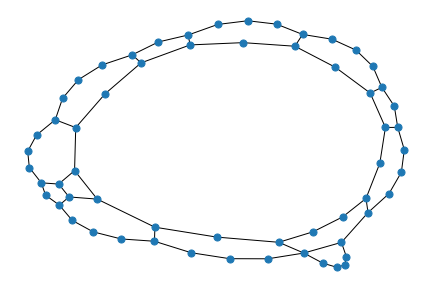
\includegraphics[scale=0.9]{data/optimal_graph.png}
    \caption{Optimal graph layout for the given connectivity structure}
    \label{fig:optimal_connectivity}
  \end{figure}


  \begin{figure}[hpb!]
    \centering
    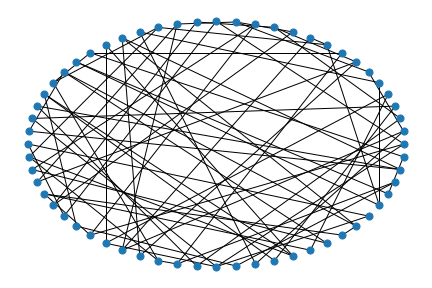
\includegraphics[scale=0.9]{data/circle_graph.png}
    \caption{Graph layout with the given circle points}
    \label{fig:circle_connectivity}
  \end{figure}


\newpage
\Q{Blind signal detection}
  \begin{solution}
    \begin{enumerate}[label=(\alph*)]
      \item
        We restate the problem in a framework we're familiar with. In fact, our goal is to:
        \begin{align*}
        \text{minimize} &  & ||w|| \\
        \text{subject to } &  & \frac{1}{T}||Aw||^2 = 1
        \end{align*}
        Note that this is equivalent to:
        \begin{align*}
        \text{minimize} &  & ||w||^2 \\
        \text{subject to } &  \frac{1}{T}||Aw||^2 = 1
        \end{align*}
        where:
        \[
          A =
            \begin{bmatrix}
              \cdots & y_1^T & \cdots \\
              \cdots & y_2^T & \cdots \\
              \cdots & \vdots & \cdots \\
              \cdots & y_T^T & \cdots
            \end{bmatrix} \in \mathbb{R}^{T \times n}
        \]
        
    \end{enumerate}
  \end{solution}

  \newpage
  \Q{Simultaneously estimating student ability and exercise difficulty}
  \begin{solution}
    Our problem is to find $\hat{G}$ which approximates $G$. In fact, what we wish to do is find the matrix $\hat{G}$ of the form:
    \[
      \hat{G} =
        \begin{bmatrix}
          \frac{1}{d_1} \\ \frac{1}{d_2} \\ \vdots \\ \frac{1}{d_m}
        \end{bmatrix}
        \begin{bmatrix}
          a_1 & a_2 & \cdots & a_n
        \end{bmatrix}
    \]
    which minimizes:
    \[
      J = \sqrt{\frac{1}{mn}\sum_{i=1}^m \sum_{j=1}^n (G_{ij} - \hat{G}_{ij})^2}
    \]
    Note that since $\sqrt{\cdot}$ is monotonic and $mn$ are constants, minimizing $J$ is equivalent to minimizing:
    \begin{align*}
      \sqrt{mn}J &= \sqrt{\sum_{i=1}^m \sum_{j=1}^n (G_{ij} - \hat{G}_{ij})^2}\\
      &= ||G - \hat{G}||_F
    \end{align*}
    As such, we can rephrase our problem as:
    \begin{align*}
      \text{minimize} && ||G - \hat{G}||_F \\
      \text{subject to} && \textbf{Rank}(\hat{G}) = 1
    \end{align*}
    From lecture, we know that this problem has the solution of:
    \[
      \hat{G} = \sigma_1 u_1v_1^T
    \]
    where the SVD decomposition of $G$ is given by:
    \[
      G = \sum_{i=1}^r \sigma_i u_i v_i^T
    \]
    where $\sigma_1 \geq \sigma_2 \geq \cdots \sigma_r > 0$. This approximation is unique of $\sigma_1 > \sigma_2$, otherwise multiple approximations achieve the same loss. 

    From the above model, we basically have what we want, expcet for the fact that we must make sure that the exam question difficulties are normalized. We therefore have:
    \begin{align*}
      d_i &= \frac{1}{u_{1i}} \left( \frac{1}{m}\sum_{j=1}^m \frac{1}{u_{1j}} \right)^{-1} \\
      &= \frac{m}{u_{1i}\sum_{j=1}^m \frac{1}{u_{ij}}} \\
      \implies 
      a_i &= \frac{m\sigma_1 v_{1i}}{\sum_{j=1}^m \frac{1}{u_{1j}}}
    \end{align*}
    Where the implication above comes from the fact that $\frac{a_i}{d_i} = \sigma_1 u_{1i} v_{1i}$. The above gives us our solution, ignoring the constraints that $a_j$ be non-negative and $d_i$ be positive.

    \item
      Carrying out the proposed method above, we obtain the normalized difficulties as the vector:
      \[
        d =
          \begin{bmatrix}
            0.943 \\
            1.278 \\
            0.902 \\
            0.920 \\
            0.773 \\
            1.042 \\
            1.143
          \end{bmatrix}
      \]
        for which the optimal value achieved is $J_{\text{opt}} = 5.675923069899214$. The ratio of $J_{\text{opt}}$ and the RMSE of $G$ is 0.35742617468116206.
  \end{solution}

  \newpage
  \Q{Square matrices and the SVD}
  \begin{solution}
    \begin{enumerate}[label=(\alph*)]
      \item False.
      \item False.
      \item False.
      \item True.
      \item False.
      \item True.
    \end{enumerate}
  \end{solution}

  \newpage
  \Q{Principal-componenets analysis of decathlon data}
  \begin{solution}
    \begin{enumerate}[label=(\alph*)]
      \item 
        A plot showing $\sigma_j$ versus $j$ is shown in Figure \ref{fig:sigma_j_vs_j}. A plot showing $p_j$ versus $j$ is shown in Figure \ref{fig:p_j_vs_j}. We also see that:
        \[
          p_2 = 0.490183068840158
        \]
      \item 
        The requested plot of the first two principal components can be seen in Figure \ref{fig:principal_components}. It's clear from the plot that some events with similarity appear to be close to each other. For example, shot put and discus are both throwing related events. Similarly, the pole value and javelin bouth require similar physical attributes. 

      \item The plot generated by the given command can be seen in Figure \ref{fig:intensity_plot}. It's clear from the plot that $v_1$ most closely appears to represent $r$, since the intensitve varies as the points move along the axis corresponding to $v_1$.

      \item The requested plots are presented in Figure \ref{fig:intensity_plot_t} and Figure \ref{fig:intensity_plot_delta}.

      From the plots, we can derive and intuitive interpretation for the first two left singular vectors of $X$. $u_1$ appears to correlate with the athletes total standardized scores, $t$. $u_2$ on the other hand appears to correlated most closely with $\delta$, which is a measure of how much better an athlete is at running/leg events (100m, long jump, 100m hurdles) compared to throwing events (shot put, discus, javelin).

    \end{enumerate}
    The code used for the above problems is now presented:
    \lstinputlisting{data/problem6.m}

  \end{solution}

  \begin{figure}[hpb!]
    \centering
    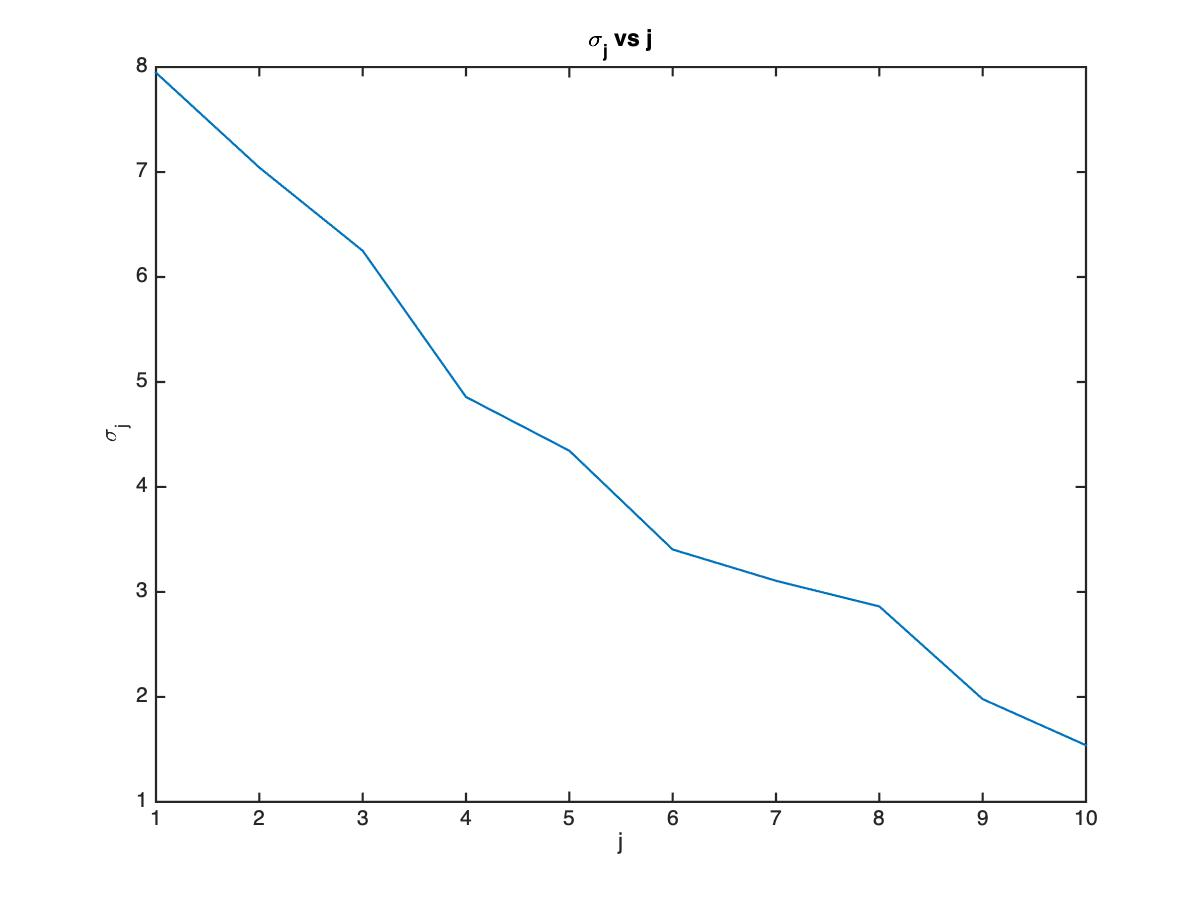
\includegraphics[scale=0.3]{data/sigma_vs_j.jpg}
    \caption{Plot of total power, $\sigma_j$, versus $j$}
    \label{fig:sigma_j_vs_j}
  \end{figure}

  \begin{figure}[hpb!]
    \centering
    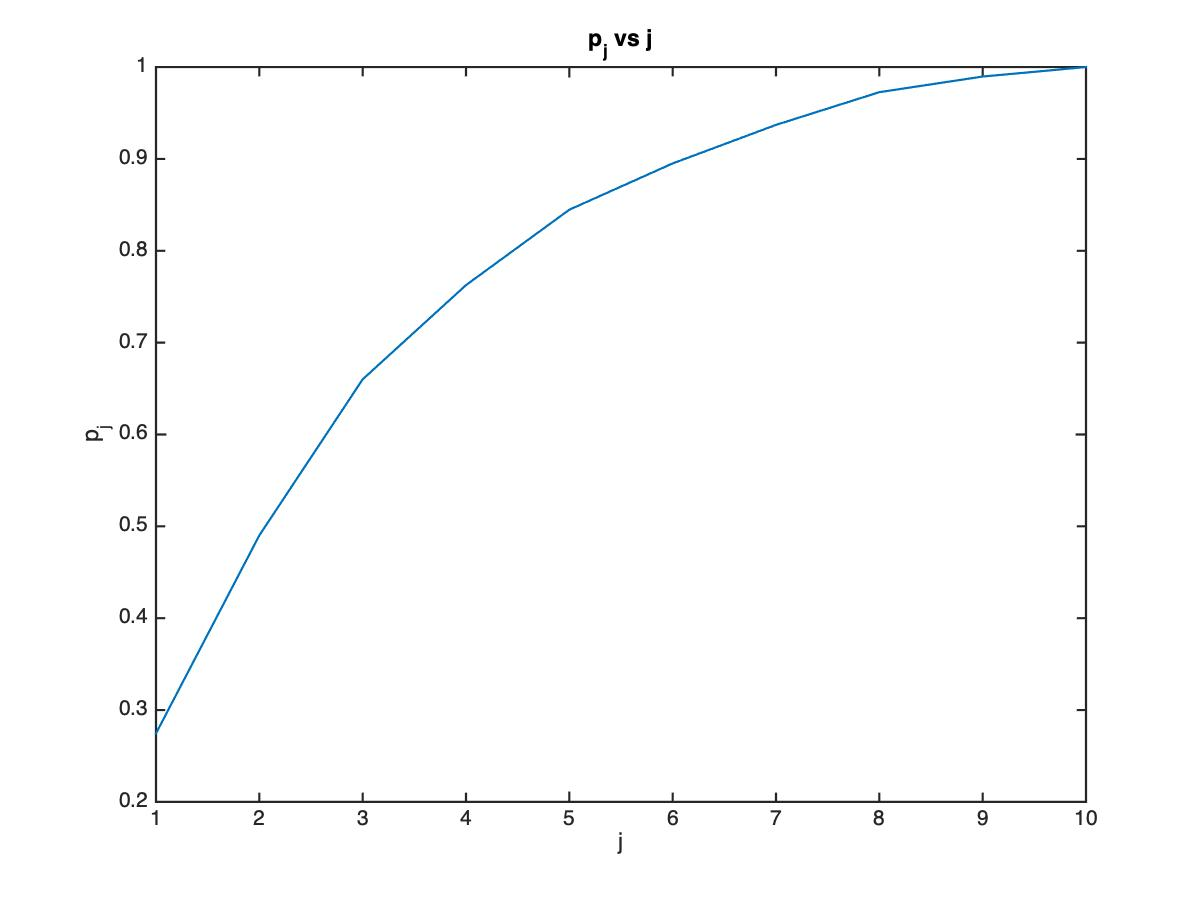
\includegraphics[scale=0.3]{data/power_vs_j.jpg}{}
    \caption{Plot of fraction of total power, $p_j$, versus $j$}
    \label{fig:p_j_vs_j}
  \end{figure}

  \begin{figure}[hpb!]
    \centering
    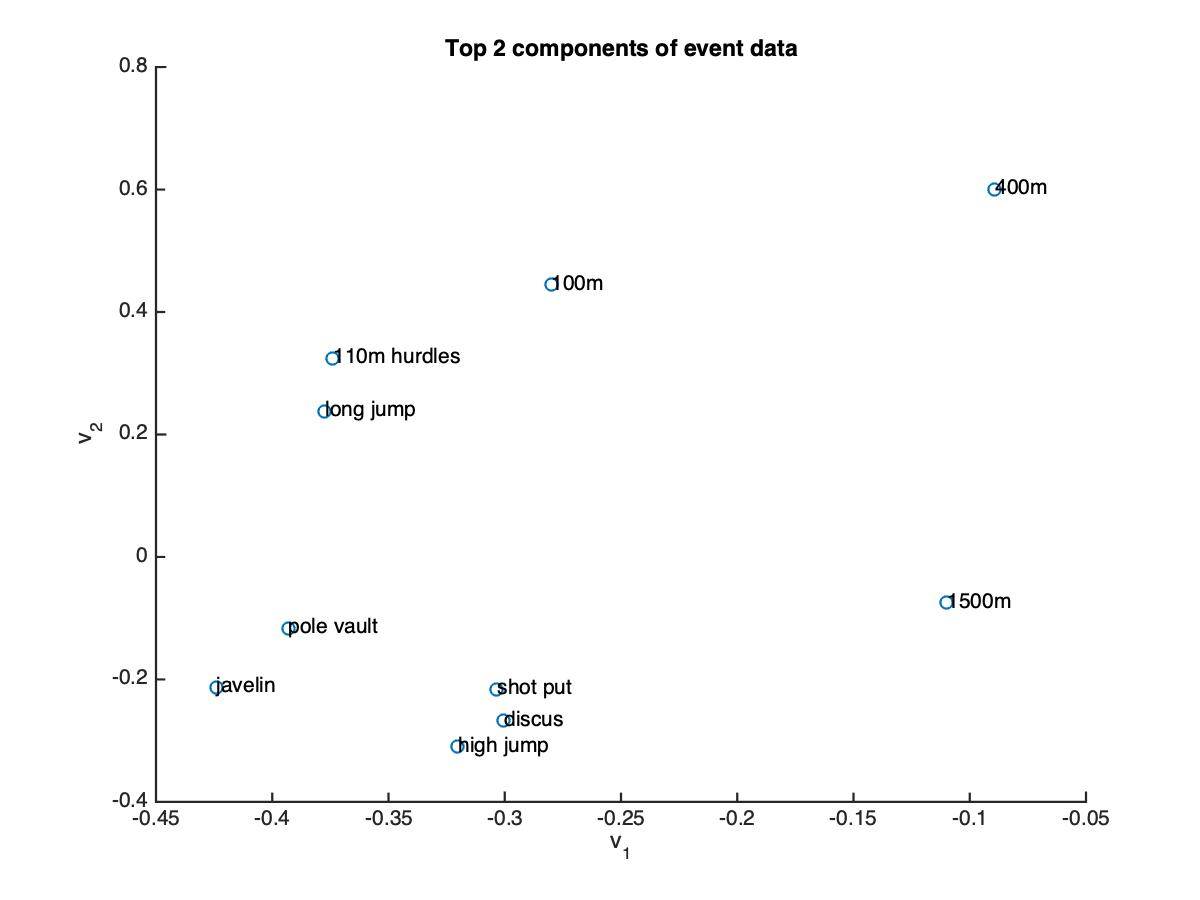
\includegraphics[scale=0.3]{data/principal_components.jpg}
    \caption{Plot of events by the first two principal components}
    \label{fig:principal_components}
  \end{figure}

   \begin{figure}[hpb!]
    \centering
    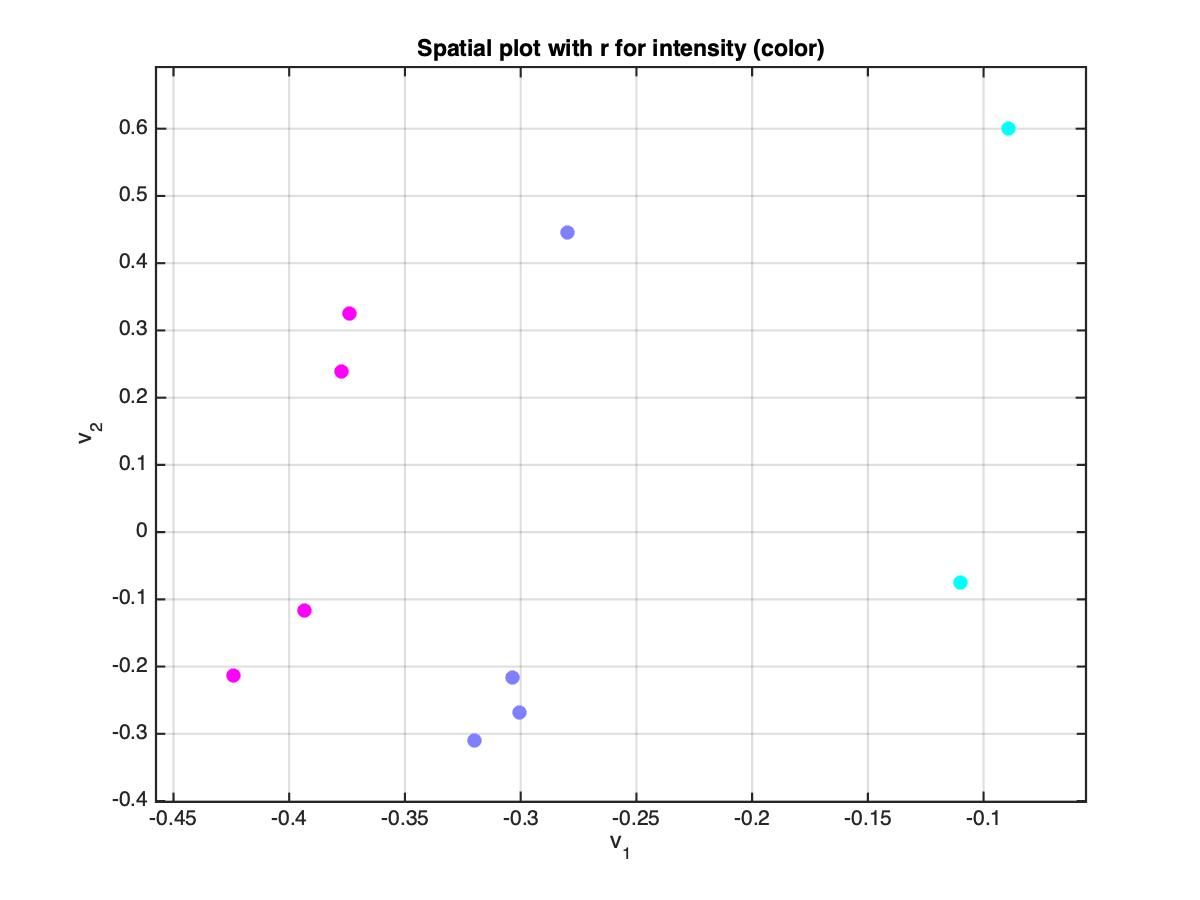
\includegraphics[scale=0.3]{data/intensity_plot.jpg}
    \caption{Plot of events colored by correlation between event and athlete's standardized test scores.}
    \label{fig:intensity_plot}
  \end{figure}

   \begin{figure}[hpb!]
    \centering
    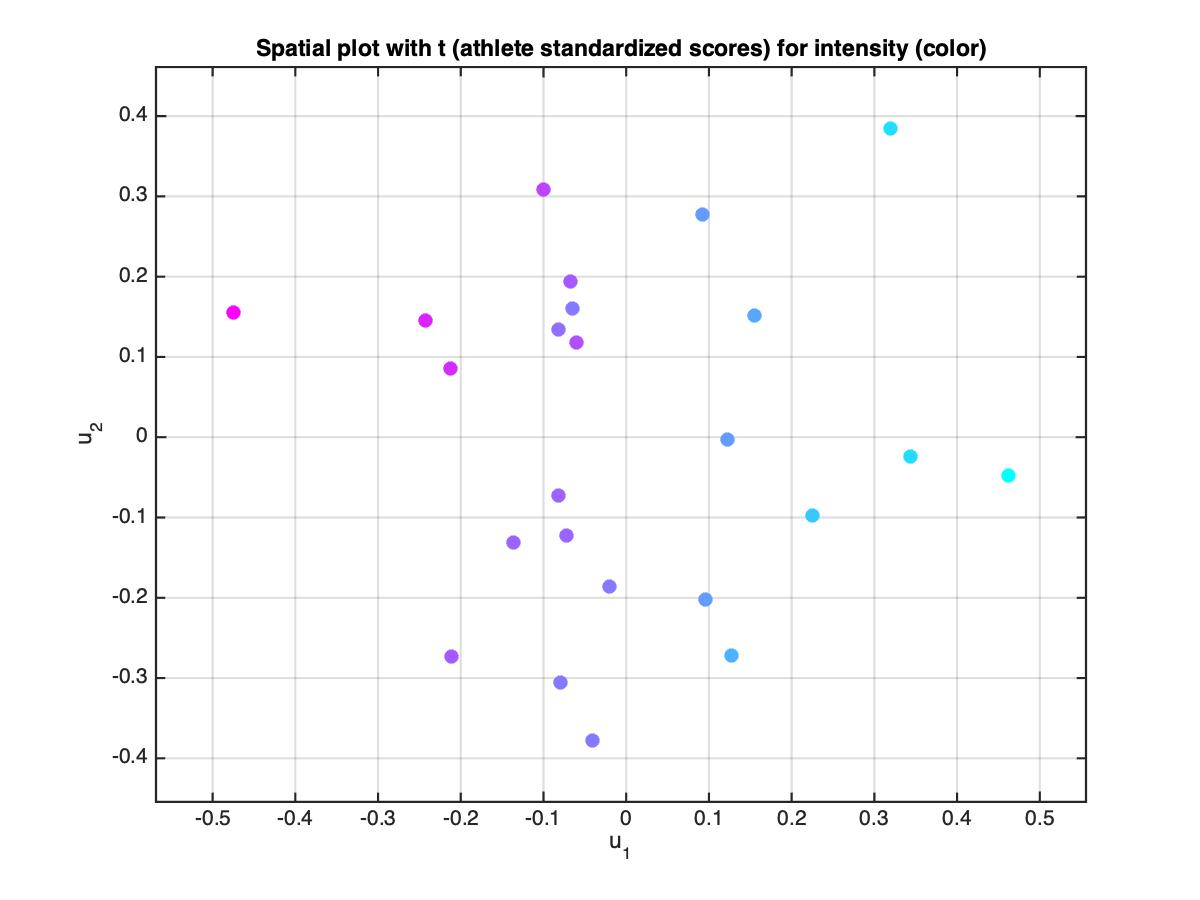
\includegraphics[scale=0.3]{data/spatial_t.jpg}
    \caption{Plot of events colored by correlation athlete's standardized test scores.}
    \label{fig:intensity_plot_t}
  \end{figure}

   \begin{figure}[hpb!]
    \centering
    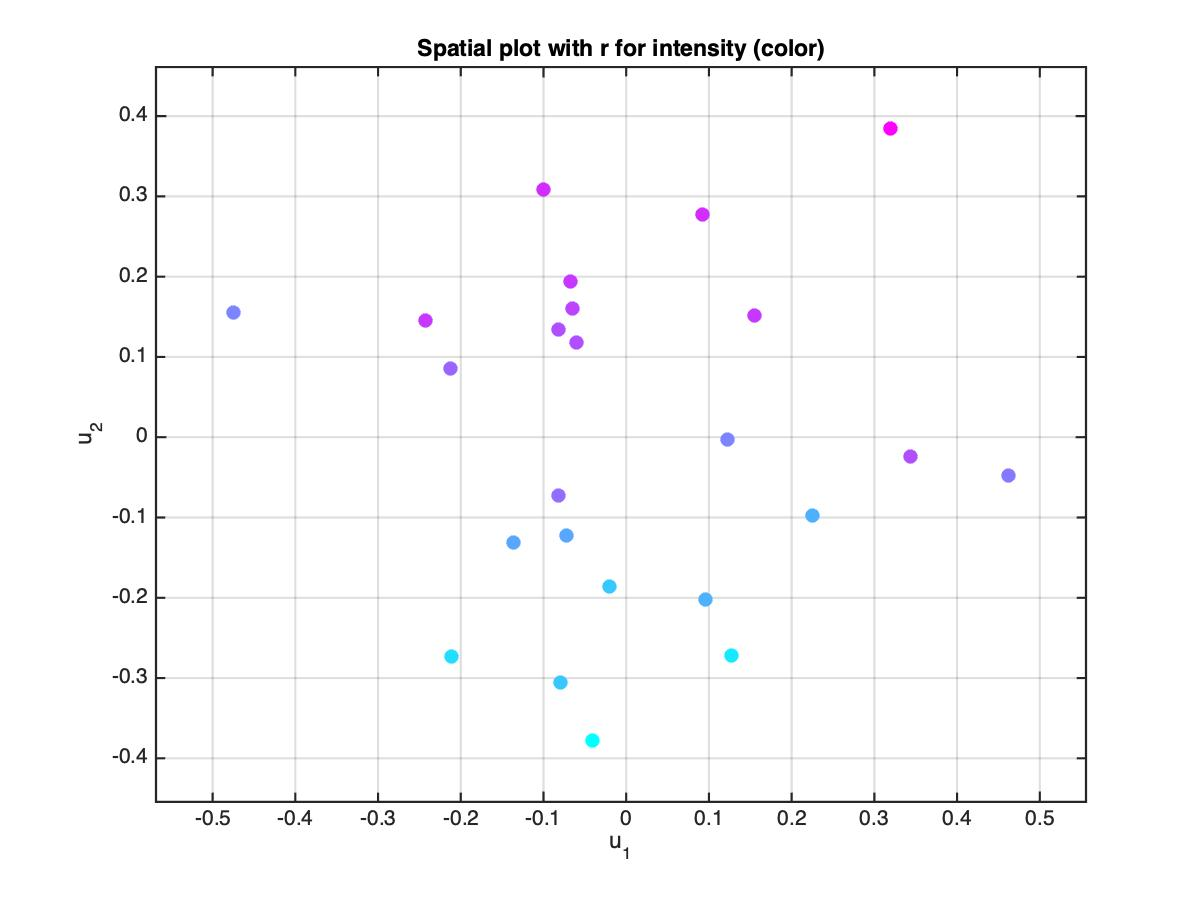
\includegraphics[scale=0.3]{data/spatial_delta.jpg}
    \caption{Plot of events colored by delta in scores between (100m, long jump, 100m hurdles) and (shot put, discus, javelin).}
    \label{fig:intensity_plot_delta}
  \end{figure}

\end{questions}


\begin{comment}
\includepdf[
    %% Include all pages of the PDF
    pages=-,
    %% make this page have the usual page style
    %% (you can change it to plain etc). By default pdfpages
    %% sets the pagecommand to \pagestyle{empty}
    pagecommand={\pagestyle{headings}}]
%% The pdf file itself
{HW6Code.pdf}
\end{comment}















\end{document}
